\section{Functionaliteit en gevaren}

\textit{In dit hoofdstuk wordt de vraag ``Hoe werken de gedistribueerde netwerken en tegen welke gevaren zijn ze bestendig?'' behandeld. Het doel van de vraag is om de werking van het gedistribueerd netwerk in kaart te brengen en tegenmaatregelen tegen aanvallen die in de functionaliteit verwerkt zitten te beschrijven.}

Deze vraag is opgesteld naar aanleiding van de criteria ``het moet resistant zijn tegen aanvallen'' die gesteld is in de opdrachtformulering zoals gegeven door Quintor, in te zien in bijlage \ref{appendix:opdrachtformulering}. Het eerste idee om deze vraag te beantwoorden was om een vergelijking te maken tussen de implementaties op het gebied van veiligheid, waarbij er onderzocht zou worden of een aanval op de implementatie uitgevoerd was. Dit zou uiteindelijk een ``beste'' implementatie opleveren die geadviseerd zou worden in het adviesrapport. Uiteindelijk is dit idee niet gebruikt omdat er een aantal redenenen zijn waarom dit niet zou werken:

\begin{itemize}
  \item \textbf{Protocol volwassenheid}
  \\ Het Bitcoin protocol bestaat al sinds 2011, terwijl het Monero protocol sinds 2014 bestaat. In het begin heeft Bitcoin waarschijnlijk veel te verduren gehad qua aanvallen, waardoor het via bovenstaande vergelijking slecht uit zou komen. Daarentegen heeft Monero gedurende de drie jaar zowel verbeteringen als lessen getrokken uit het Bitcoin protocol.

  \item \textbf{Adoptie van de technologie}
  \\ Proof of Work implementaties zijn vatbaar voor een \gls{majority_attack}, waarbij een gebruiker 51\% van de rekenkracht binnen het netwerk in handen moeten hebben om transacties in de Blockchain te registreren zonder dat er validatie te pas komt. Hoe minder gebruikers, hoe minder de benodigde rekenkracht om dit uit te voeren.
\end{itemize}

Om deze reden is er besloten om met de Blockchain expert over de aanpak en uiteindelijke doel van deze vraag te discussiëren, wat ertoe heeft geleid dat de focus van de vraag veranderd is van een vergelijking doen op basis van de veiligheid, het een meer beschrijvende vorm heeft gekregen waar er gekeken wordt naar componenten van het netwerk: discovery protocol, hoe informatie verstuurd wordt tussen twee \glspl{node} en wanneer mogelijk de knelpunten met betrekking tot aanvallen binnen deze componenten.

\newpage
\subsection{Aanpak}

\begin{wrapfigure}[14]{r}{0.6\textwidth}
  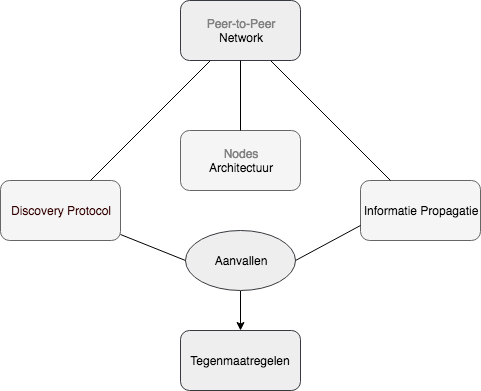
\includegraphics[width=0.6\textwidth]{figures/uitwerking_functionaliteit}
  \caption[Opbouw beantwoording ``Functionaliteit en gevaren'']{Componenten en termen die als leidraad gebruikt zijn om het resultaat te beschrijven.}
  \label{opbouw:functionaliteit}
\end{wrapfigure}

In fig. \ref{opbouw:functionaliteit} is te zien welke componenten er gebruikt zijn om de benodigde informatie te vinden. Hieronder is de werkwijze en denkwijze uitgeschreven per individueel onderdeel.

\subsubsection{Aanvallen}

Allereerst is er begonnen met het zoeken naar de verschillende aanvallen die mogelijk zijn op Blockchain implementaties. Binnen het gesprek met de Blockchain Expert is hierbij het woord threat model gevallen, en zijn er een aantal aanvallen aan bod gekomen:

\begin{itemize}
  \item \textbf{Eclipse attack}
  \\ Meer informatie en de definitie van een eclipse attack is gevonden in de studie van \cite{heilman2015eclipse}.

  \item \textbf{Majority attack}
  \\ De majority attack staat beschreven op de wiki van Bitcoin, waarbij er uitgelegd wordt wat het is, wat er mee mogelijk is en waarom het bijna niet uit te voeren is.

  \item \textbf{Denial of Service}
  \\ Bij Denial of Service gaat het om meerdere manieren om de uitvoering van processen binnen het netwerk te verstoren, waardoor er niet een specifieke bron te vinden is voor alle mogelijke aanvallen.

  \item \textbf{Sybil attack}
  \\ Voor het beschrijven van de sybil attack in relatie tot Blockchain is er gebruik gemaakt van de studie gedaan door \cite{conti2017survey}.

  \item \textbf{Double spending}
  \\ Informatie double spending is gevonden in de studie van \cite{karame2012double}.
\end{itemize}

Een van de knelpunten bij het beschrijven van een aanval was een studie vinden die aantoonde wat het gevolg ervan was binnen een Blockchain implementatie.

\subsubsection{Network}

Voor het beschrijven van de verschillende netwerken is er gebruikt gemaakt van niet wetenschappelijke bronnen zoals wiki's of blogs. De reden hiervoor is dat een whitepaper van een Blockchain implementatie zelden de architectuur van het netwerk beschrijft. Deze informatie is dan ook gebruikt om de verschillende componenten van het netwerk te beschrijven.

\subsection{Conclusie}

\paragraph{Bitoin} Het netwerk van Bitcoin communiceert via TCP/IP en maakt gebruik van bootstrap nodes waarmee connectie wordt gemaakt op het moment dat een nieuwe deelnemer het netwerk wilt toetreden. Informatie wordt verstuurd door een voorafgedefinieerde set aan berichttypes: \textit{inv}, \textit{tx}, \textit{block}, \textit{getdata}, waarbij een \textit{inv} bericht gebruikt wordt ter inventarisatie over de beschikbaarheid van data, \textit{tx} bericht om een transactie te versturen, \textit{block} bericht om een block te versturen, \textit{getdata} bericht om data op te vragen. \\ \\ Op het Bitcoin netwerk zijn meerdere aanvallen in de loop der jaren uitgevoerd en geïdentificeerd, een studie uit 2015 gedaan door \cite{heilman2015eclipse} toont aan dat het Peer Discovery mechanisme vatbaar is voor een Sybil Attack. \cite{nakamoto2008bitcoin} stelt dat de voordelen van het uitvoeren van een majority attack niet opweegt tegen de kosten voor de benodigde hardware om de rekenkracht te behalen. \cite{eyal2014majority} beschrijft dat het niet nodig is om een merendeel van de rekenkracht te bezitten en introduceert de aanval \gls{selfish_mining}.

\newpage
\paragraph{Cardano} Het netwerk van Cardano communiceert via TCP/IP en maakt gebruik van het Kademlia protocol waardoor het maar nodig is om één bootstrap node te gebruiken om het netwerk toe te treden. De achterliggende structuur van Kademlia is een Binary Tree waarbij de positie van een deelnemer in de Binary Tree bepaald wordt door een unieke prefix van de identificatiecode. Het protocol garandeert dat een deelnemer in verbinding staat met ten minste één andere deelnemer. Informatie wordt uitgewisseld door drie abstracte berichttypes: \textit{inv}, \textit{req}, en \textit{data}. Het \textit{inv} bericht wordt gebruikt om aan te geven dat er data beschikbaar is, het \textit{req} bericht wordt gebruikt om beschikbare data op te vragen en het \textit{data} bericht wordt vervolgens gebruikt om de data te versturen. \\ \\ Implementaties die gebruik maken van \acrshort{PoS} zijn afhankelijk van de manier waarop een leiderschapsverkiezing wordt gesimuleerd, waarbij er grote kans is dat het gevoelig is voor beïnvloedingen van kwaadwillende deelnemers in het netwerk in de vorm van een Sybil Attack. Cardano heeft een zwak punt in het Kademlia netwerk geïdentificeerd waardoor het mogelijk zou zijn om Eclipse Attack uit te voeren.

\paragraph{Monero} Het netwerk van Monero maakt gebruik van het \acrfull{I2P} protocol, dat zowel UDP/IP als TCP/IP ondersteund. Om het netwerk toe te treden wordt er gebruik gemaakt van bootstrap nodes die vastgelegd zijn in de broncode. Communicatie wordt gedaan door middel van \Glspl{tunnel}, waarbij elke deelnemer twee \Glspl{tunnel}, een inkomende en een uitgaande, heeft voor elke connectie.

\paragraph{EOS} \textit{Ten tijde van het onderzoek is er geen technische beschrijving beschikbaar over het netwerk component van EOS.}




